\documentclass{beamer}
\usepackage{color}
\usepackage{listings}
\usepackage{verbatim}
\usepackage{graphicx}
\usepackage{multicol}
\usepackage[utf8]{inputenc}
\usepackage{amsmath}
\usepackage{graphicx}
\usetheme{Warsaw}
\title{Bachelor-Thesis Proposal}
\subtitle{Simulation of the RoboCup Logistic League with Fawkes and Gazebo for Multi-Robot Coordination Evaluation}
\author {Frederik Zwilling}
\institute{RWTH Aachen}
\date{23.07.13}
\subject{Multi-Robot Simulation}

\begin{document}
\frame{\titlepage}

%Übersicht
\begin{frame}
\frametitle{Overview}
\begin{enumerate}
\item Motivation
\item \textcolor{gray}{Background}
\item \textcolor{gray}{Related Work}
\item \textcolor{gray}{Goals}
\item \textcolor{gray}{Evaluation}
\item \textcolor{gray}{Conclusion}
\end{enumerate}
\end{frame}

%Motivation
\begin{frame}
\frametitle{Motivation}
\begin{multicols}{2}
Autonomous Multi-Robot Systems are useful:
\begin{itemize}
\item<1-> in warehousing
\item<2-> in logistics
\item<3-> and many other domains
\end{itemize}
\begin{figure}
\only<1>{\includegraphics[width=130pt,heigth=80pt]{pics/kiva.jpg}\\}
\only<2>{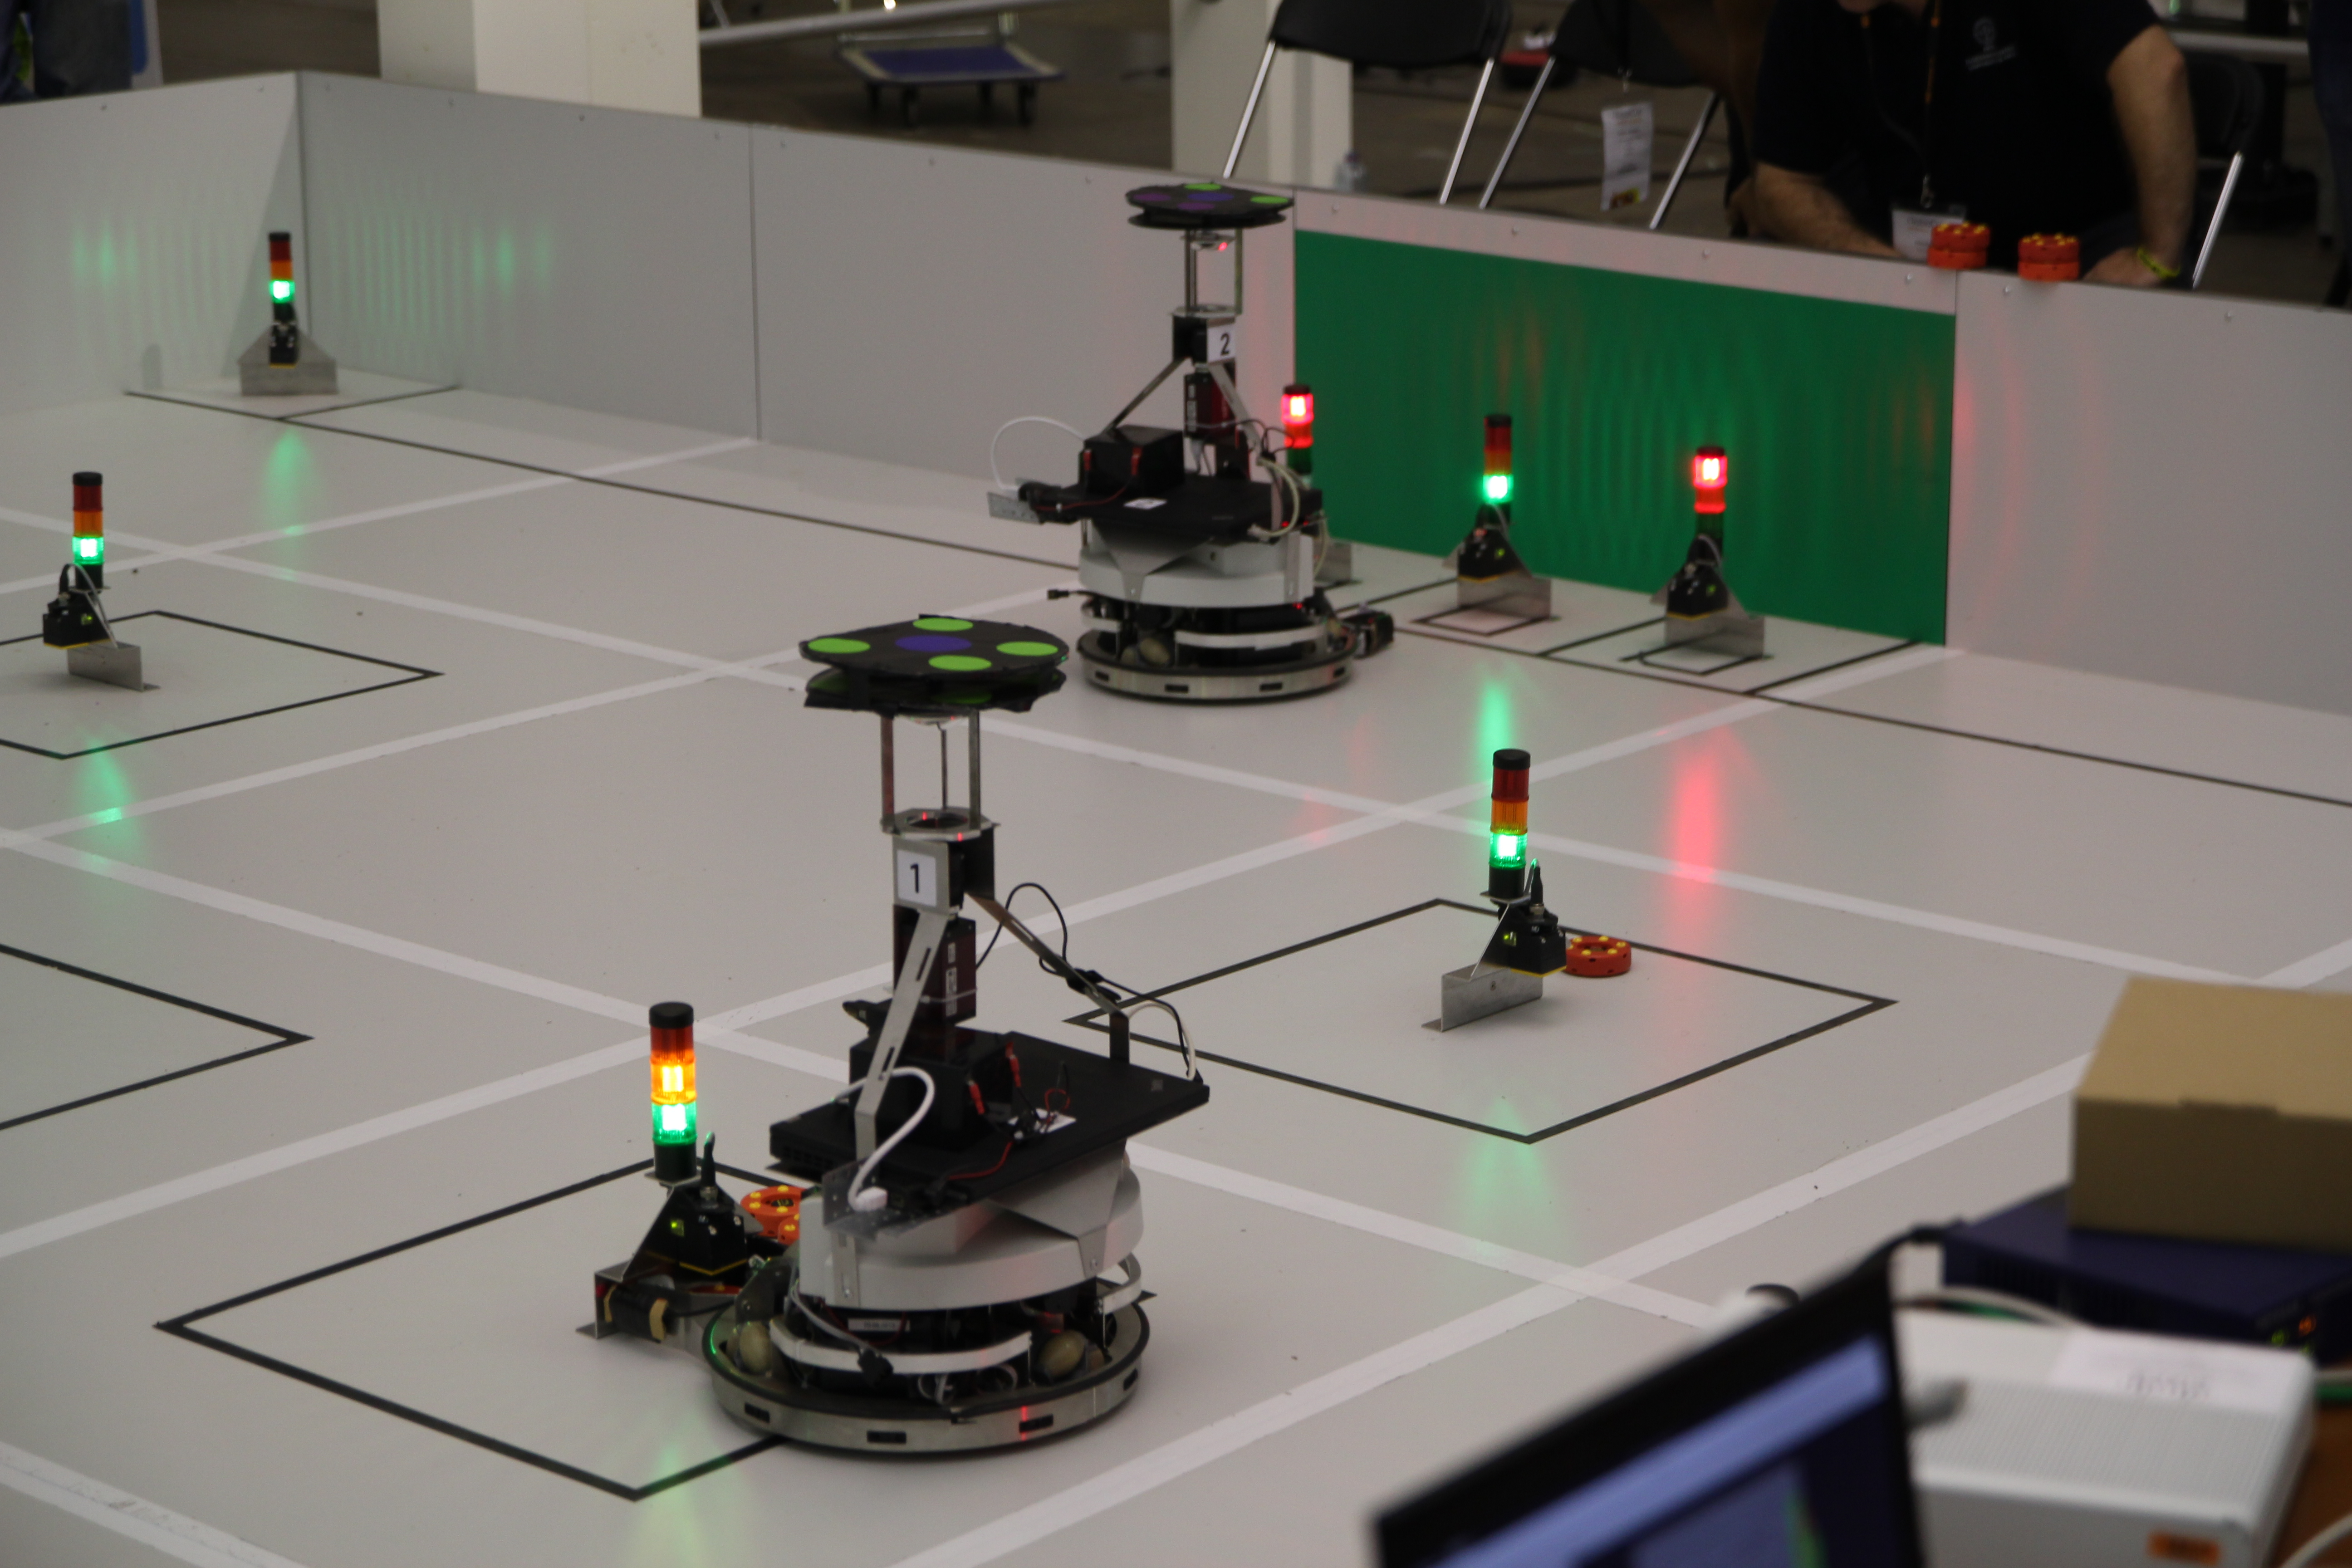
\includegraphics[width=130pt,heigth=80pt]{pics/llsf.jpg}\\}
\only<3->{\includegraphics[width=130pt,heigth=80pt]{pics/rimes.jpg}\\}
\end{figure}
\end{multicols}
\pause
\begin{multicols}{2}
and difficult to test and evaluate because of:
\begin{itemize}
\item<4->
\item<5->
\item<6->
\end{itemize}
\end{multicols}
\end{frame}


\end{document}
